%%=============================================================================
%% CAPITULO 2 -- REFERENCIAL TEORICO
%%=============================================================================

\section{Referencial teórico}

A classificação com opção de rejeição, chamada de classificação seletiva,
troca cobertura por acurácia: ao recusar os casos mais duvidosos, o
classificador reduz o erro entre os casos que decide. \citeonline{elyaniv2010}
chamam esse compromisso de troca risco-cobertura e o tomam como objeto central
da teoria. A Figura~\ref{fig:fluxo-seletiva} resume o mecanismo: um
classificador propõe a classe e uma função de seleção decide se a proposta é
aceita ou encaminhada a uma pessoa. Geifman e El-Yaniv apresentam a motivação
dessa linha de pesquisa nos seguintes termos:

\begin{citacao}
While self-awareness remains an illusive, hard to define concept, a
rudimentary kind of self-awareness, which is much easier to grasp, is the
ability to know what you don't know, which can make you smarter. The subfield
dealing with such capabilities in machine learning is called selective
prediction (also known as prediction with a reject option), which has been
around for 60 years. \parencite[p.~1]{geifman2017}
\end{citacao}

\begin{figure}[htb]
  \caption{Fluxo de uma classificação seletiva}
  \label{fig:fluxo-seletiva}
  \centering
  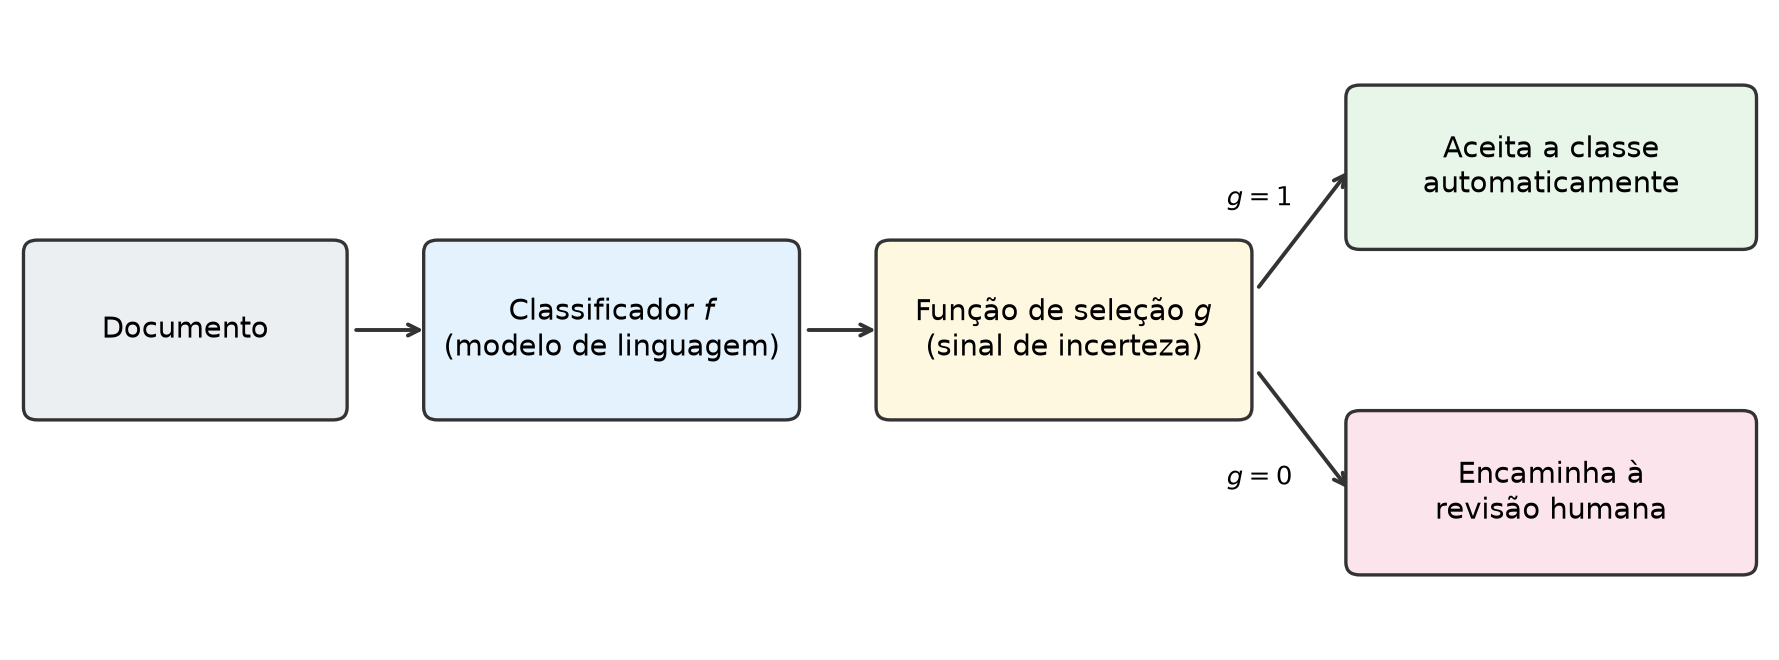
\includegraphics[width=0.95\textwidth]{figuras/fluxo-classificacao-seletiva.png}
  \fonte{Elaborado pelo autor com base em Geifman e El-Yaniv (2017).}
\end{figure}

Para que a função de seleção funcione com modelos de linguagem, é preciso que
eles carreguem algum sinal confiável sobre a própria chance de erro.
\citeonline{kadavath2022} mostram que modelos maiores são bem calibrados em
questões de múltipla escolha e de verdadeiro ou falso quando recebem o formato
adequado, e propõem dois sinais de autoavaliação, descritos na
Tabela~\ref{tab:sinais-incerteza}. Esses sinais são candidatos naturais à
função de seleção da Figura~\ref{fig:fluxo-seletiva}, desde que se verifique
se continuam informativos fora dos conjuntos de teste em que foram propostos.

\begin{table}[htb]
  \caption{Sinais de autoavaliação de modelos de linguagem}
  \label{tab:sinais-incerteza}
  \centering
  \begin{tabular}{lll}
    \toprule
    \textbf{Sinal} & \textbf{Pergunta que responde} & \textbf{Quando é obtido} \\
    \midrule
    P(True) & A resposta proposta está correta? & Depois de o modelo responder \\
    P(IK)   & O modelo sabe responder?          & Antes de qualquer resposta \\
    \bottomrule
  \end{tabular}
  \fonte{Elaborado pelo autor com base em Kadavath et al. (2022).}
\end{table}
